\documentclass[a4paper,10pt]{article}
\usepackage[utf8]{inputenc}
\usepackage[T1]{fontenc}	
\usepackage[italian]{babel}

\usepackage{amsmath}
\usepackage{amsfonts}
\usepackage{amssymb}
\usepackage{graphicx}

\usepackage[left=2cm,right=2cm,top=2cm,bottom=2cm]{geometry}
\geometry{a4paper}

\usepackage{booktabs}
\usepackage{verbatim}
\usepackage{subfig}

\usepackage[cdot, thickqspace, squaren]{SIunits}
\usepackage{float}

% macro
\def\code#1{\texttt{#1}}

\title{Esperienza di Ottica 2}
\author{Gruppo BL \\ Candido Alessandro, Luzio Andrea, Mazziotti Fabrizio}

\begin{document}

\maketitle

\section{Scopo}
L'esperienza è divisa in due parti:
\begin{itemize}
	\item nella prima parte si vuole misurare la lunghezza d'onda di un laser ad He-Ne.
	\item nella seconda parte si vuole misurare la lunghezza d'onda della radiazione emessa da una lampada al mercurio.
\end{itemize}

\section{Esperienza A: Misura della lunghezza d'onda di un laser ad He-Ne}

\subsection{Strumentazione}

\begin{itemize}
	\item spettroscopio a prisma:
	\item Laser ad He-Ne;
	\item Schermo per visualizzare la figura di diffrazione;
	\item Specchio per deviare il raggio laser sullo schermo;
	\item Righello graduato di un calibro ventesimale;
	\item riga;
	\item torcia.
\end{itemize}

\subsection{Misura della lunghezza d'onda del laser ad He-Ne}
In questa prima parte dell'esperienza si vuole misurare la lunghezza d'onda di un laser ad He-Ne. Per fare ciò si è indirizzato il laser, attraverso uno specchio, sul righello graduato di un calibro ventesimale, utilizzando queste righe come un reticolo di diffrazione. Poiché il passo $d$ di questo reticolo( d = 1 mm) è molto più grande della lunghezza d'onda attesa ($\lambda_{att} \sim$ 650 nm), si è fatto in modo che il fascio laser incida sul righello con un angolo di circa $\pi/2$, altrimenti non si avrebbe modo di apprezzare la figura di diffrazione.
Questa figura di diffrazione si può osservare su un opportuno schermo vicino al banco di lavoro su cui è fissato un foglio di carta per la presa dati.
L'equazione che lega la posizione dei massimi di diffrazione al passo reticolare $d$ e all'angolo di incidenza $\theta_i$ è

\begin{equation}
d(sin\theta_i - sin\theta_d)= m\lambda
\label{reticolo}
\end{equation}

dove $\theta_d$ è l'angolo di riflessione.
Una rappresentazione schematica di ciò che accade è mostrata in figura \figurename{~\ref{fig:espa}.

\begin{figure}[H]
	\centering
	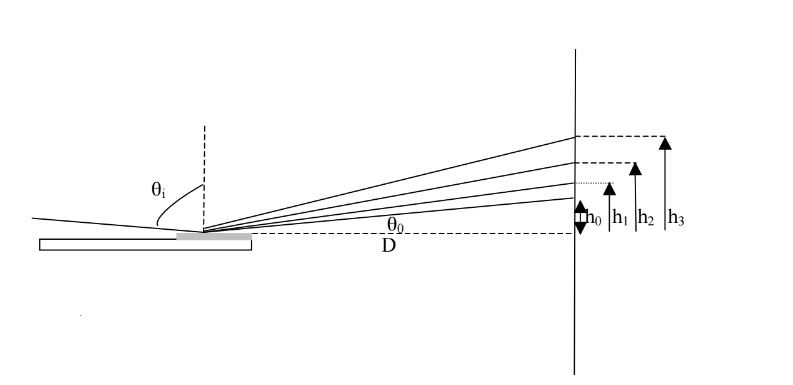
\includegraphics[width=0.7\textwidth]{../grafici/espa.png}
	\caption{Schema di un raggio incidente sul calibro e della figura di diffrazione che si viene a formare. $\theta_i$ è l'angolo di incidenza, D la distanza del reticolo dallo schermo, $\theta_n$ e $h_n$ sono rispettivamente il complementare dell'angolo di riflessione e la distanza dei vari massimi dalla quota del calibro sullo schermo.}
	\label{fig:espa}
\end{figure}

Per prima cosa si è trovata sullo schermo la quota del calibro, poiché tutte gli ordini di diffrazione devono essere riferiti a questa misura che rappresenta lo zero sull'asse dello schermo. Tale quota si è trovata misurando il punto intermedio tra la luce non riflessa dal calibro (cioè quella che si vede bene in assenza di esso) e l'ordine zero di diffrazione, che nella figura \figurename{~\ref{fig:espa} corrisponde alla quota $h_0$. Inoltre dalla posizione dell'ordine zero (m = 0), utilizzando la formula \ref{reticolo}, si può trovare l'angolo di incidenza $\theta_i$. Successivamente si sono presi gli altri ordini e, dalla misura della distanza di essi dallo zero dell'asse precedentemente trovato ($h_n$), si sono trovati i complementari degli angoli di riflessione utilizzando le formule

\begin{align*}
sin\theta_{d,n} = sin(\pi/2 - \theta_n)
\end{align*}
\begin{equation}
\theta_n = arctg(h_n/D)
\end{equation}

dove D è la distanza del calibro dallo schermo, misurata mediante un metro a nastro.


ERRORI, QUANTO VALE D
Per quanto riguarda gli errori associati alle misure, si sono effettuati i seguenti accorgimenti:
\begin{itemize}
\item 
\end{itemize}

Effettuando i calcoli si ottiene come angolo di incidenza $\theta_i = rad$, risultato molto vicino a $\pi/2 rad$, come ci si poteva aspettare in seguito alle condizioni in cui ci si è posti per l'esperienza. I vari valori delle altezza $h_n$ rispetto allo zero dello schermo e degli angoli di riflessione sono riportati in \tablename{~\ref{tab:data}.

TABELLA DATI



Riscrivendo l'equazione \ref{reticolo} come
\begin{align*}
sin\theta_d = - m(\lambda/d) + sin\theta_i
\end{align*} 
  
si è effettuato un fit lineare utilizzando come variabile dipendente $\sin\theta_d$ e come variabile indipendente $m$. Dal valore $d$ del passo reticolare del calibro si è quindi ottenuta una misura della lunghezza d'onda del laser ad He-Ne. I risultati del fit sono riportati in \tablename{~\ref{tab:fita}.


TABELLA

Dai risultati del fit si può osservare come il valore di $\sin\theta_i$ sia compatibile con la misura effettuata precedentemente e con le condizioni scelte nell'esperienza riguardo quest'angolo.
Il valore della lunghezza d'onda del laser ad He-Ne è dell'ordine del valore atteso (650 nm), ma non è perfettamente compatibile PERCHE'...
Il $\chi^2$ è sottostimato. Si ritiene che ciò sia dovuto al fatto che tutti gli errori considerati nell'elaborazione dati sono errori strumentali e non statistici, che quindi risultano essere inevitabilmente una sovrastima dell'errore da attribuire alla misura per effettuare il fit.


\section{Esperienza B: Misura della lunghezza d'onda della radiazione emessa da una lampada al mercurio mediante l'interferometro di Michelson}






\end{document}